\documentclass[main.tex]{subfiles}
\begin{document}
% 5
\section{Hermitian Operators}
First, some basic facts dealing 
with normed vector spaces and Hilbert spaces.
%
%                  5.1
%
\begin{psec}{5.1}%
Let $E$ and $F$ be vector spaces,
endowed with norms $\|\cdot\|_E$ and $\|\cdot\|_F$, respectively.
\begin{enumerate}
\item \label{5.1-1}
Let $T$ be a linear map $E\ra F$.

If there exists a number $c\in [0,\infty)$ such that
\begin{equation*}
\|Tx\|_F \ \leq \ c\,\|x\|_E \qquad (x\in E)
\end{equation*}
then $\|Tx-Ty\|_F \leq \|x-y\|_E\quad (x,y\in E)$,
so that~$T$ is continuous
(relative to the metrics induced by the norms).

On the other hand,
if no such~$c$ exists,
$T$ is \emph{not} continuous.
Indeed,
for every $n\in\N$
there then exists an~$x_n$ in~$E$
with $\|T x_n\|_F > n \|x_n\|_E$.
Then~$x_n\neq 0$, so $\|x_n\|_E\neq 0$.
Putting $y_n:=(n\|x_n\|_E)^{-1}x_n$
we get $y_n\ra 0$
but not $Ty_n\ra 0=T0$.
%
\item \label{5.1-2}
The continuous linear maps $E\ra F$ form a vector space
\begin{equation*}
\Lin(E,F)\htam{.}
\end{equation*}
With every $T\in\Lin(E,F)$ 
we associate a nonnegative number $\| T \|$ by
\begin{equation*}
\|T\| = \inf \bigl\{ c\colon 
\|Tx\|_F \leq c\,\|x\|_E\htam{ for all }x\in E\bigr\}\htam{.}
\end{equation*}
Then
\begin{equation*}
\|Tx\|_F\ \leq\ \|T\|\,\|x\|_E \qquad (T\in\Lin(E,F),\ x\in E)\htam{.}
\end{equation*}
It is not difficult to verify
that~$\|\cdot\|$ is a norm on $\Lin(E,F)$.
It is called the \keyword{operator norm}.
An important fact:
\statement{$\Lin(E,F)$ is complete relative to the operator norm
in case~$F$ is complete relative to~$\|\cdot\|_F$.}
\end{enumerate}
\end{psec}
%
%                  5.2
%
\begin{psec}{5.2}%
An inner product $\left<\cdot,\cdot\right>$
on a vector space~$H$
induces a norm~$\|\cdot\|$:
\begin{equation*}
\|x\|:=\sqrt{\left<x,x\right>}\qquad(x\in H)
\end{equation*}
satisfying the \keyword{Cauchy--Schwarz Inequality}
\begin{equation*}
\left|\left<x,y\right>\right| \ \leq\ \|x\|\,\|y\|\qquad(x,y\in H)\htam{.}
\end{equation*}

Relative to this norm,
for each $x\in H$
the function $y\mapsto \left<x,y\right>$ is continuous
(since $\left|\left<x,y_1\right>-\left<x,y_2\right>\right|
\leq\|x\|\,\|y_1 - y_2\|$ for all $y_1,y_2$).

The inner product space $(H,\left<\cdot,\cdot\right>)$ 
is called a \keyword{Hilbert space}
if~$H$ is complete relative to the inner product norm.
\end{psec}
%
%                  5.3
%
\begin{psec}{5.3}%
Let~$E$ be a vector space.
\begin{enumerate}%
\item\label{5.3-1}%
A \keyword{semi-inner product} on~$E$ is a function $[\cdot,\cdot]$
on $E\times E$ satisfying
\begin{enumerate}[label={},itemindent=2em,labelindent=2em]
\item $y\mapsto [x,y]$ is linear for each $x$;
\item $[x,y]=[y,x]\qquad(x,y\in E)$;
\item $[x,x]\geq 0\qquad(x\in E)$.
\end{enumerate}
These properties suffice to 
imply a \keyword{Cauchy--Schwarz Inequality}:
\begin{equation*}
|[x,x]|\ \leq\ \sqrt{[x,x]}\,\sqrt{[y,y]}
\end{equation*}

For example,
let $E$ be the space of all Riemann integrable functions
on the interval~$[0,1]$, with
\begin{equation*}
[f,g]\ :=\ \int_0^1 f(x)g(x)\,\mathrm{d}x\htam{.}
\end{equation*}
%
\item \label{5.3-2}
Let $[\cdot,\cdot]$ be such a semi-inner product on~$E$.
The elements~$x$ of~$E$ for which $[x,x]=0$
form a linear subspace~$D$ of~$E$.
Make the quotient vector space~$E/D$
and the quotient map $Q\colon E\ra E/D$.
Then the formula
\begin{equation*}
\left< Qx,Qy \right> = [x,y]\qquad (x,y\in E)
\end{equation*}
determines a bona fide inner product on~$E/D$.
\end{enumerate}
\end{psec}

\noindent {\sc From here on in this chapter
$H$ is a Hilbert space.}

%
%                  5.4
%
\begin{psec}{5.4}{Definition}
A map $T\colon H\ra H$ is called a \keyword{Hermitian operator} if
\begin{equation*}
\left\{\ 
\begin{alignedat}{2}
&T\htam{ is linear and continuous;} \\
&\htam{if }x,y\in H\htam{, then }
\left<Tx,y\right>=\left<x,Ty\right>\htam{.}
\end{alignedat}
\right.
\end{equation*}
(It can be proved that a linear $T\colon H\ra H$ 
with $\left<Tx,y\right>=\left<x,Ty\right>$
for all~$x$ and~$y$ must be continuous.)

The Hermitian operators form a vector space
\begin{equation*}
\mathscr H\htam{.}
\end{equation*}

$\mathscr H$ is a linear subspace of $\Lin(H,H)$,
closed under the operator norm. (See~\ref{5.1}\ref{5.1-2}.)
Indeed,
if $(T_n)_n$ is a sequence in~$\mathscr H$,
converging to an element~$T$ of $\Lin(H,H)$
in the sense of the operator norm,
then $T_n x\rightarrow Tx$ for every $x\in H$,
so $\left< Tx, y \right> 
= \lim\left< T_n x, y \right>
= \lim\left< x, T_n y \right>
= \left< x, Ty \right>\quad (x,y\in H)$.
\end{psec}

In \ref{5.5}\ref{5.5-1} we will see
that the product of two Hermitian operators
need not be Hermitian.
%
%                  5.5
%
\begin{psec}{5.5}{Examples}
\begin{enumerate}
\item \label{5.5-1}
$\R^2$ is a Hilbert space under the standard inner product.
All linear maps $\R^2\ra\R^2$ are continuous.
If we identify a linear map $\R^2\ra\R^2$ with its matrix,
the Hermitian operators in~$\R^2$ are precisely the matrices
\begin{equation*}
\begin{pmatrix}
a & b \\
b & c 
\end{pmatrix}\htam{.}
\end{equation*}
The identity
\begin{equation*}
\begin{pmatrix} 1 & 0 \\ 0 & 0 \end{pmatrix}
\begin{pmatrix} 1 & 1 \\ 1 & 1 \end{pmatrix}
=
\begin{pmatrix} 1 & 1 \\ 0 & 0 \end{pmatrix}
\end{equation*}
shows that a product of two Hermitian operators
may not be Hermitian.
%
\item \label{5.5-2}
By $\ell^2$ we denote the space of all real number sequences
$x=(x_n)_n$ for which $\sum x_n^2<\infty$.
This~$\ell^2$ is a Riesz ideal in~$\ell^\infty$.

It is not quite trivial to prove that~$\ell^2$
is a Hilbert space under
\begin{equation*}
\left<x,y\right>\ :=\ \sum_{n=1}^\infty x_n y_n \qquad (x,y\in\ell^2)\htam{.}
\end{equation*}

Continuous linear maps $\ell^2\ra\ell^2$
can be presented by infinitely large matrices;
Hermitian operators correspond to symmetric matrices.
(Not every infinitely large matrix denotes a map $\ell^2\ra\ell^2$.)
%
\item \label{5.5-3}
On $\Cont{[0,1]}$ we have the inner product
\begin{equation*}
\left< f,g\right>\ = \ \int_0^1 f(x)g(x)\,\mathrm{d}x
\qquad(f,g\in\Cont{[0,1]}\,)\htam{.}
\end{equation*}
Under this inner product,
$\Cont{[0,1]}$ is not complete.
However,
as a metric space
(with the inner product metric),
it has a completetion.
For esoteric reasons of our own
we call this completion~$\Leb^2[0,1]$.
It turns out to be possible (and not too difficult)
to extend the addition, scalar multiplication and inner product
of $\Cont{[0,1]}$ to $\Leb^2[0,1]$,
rendering $\Leb^2[0,1]$ a Hilbert space.
(In a later chapter we will see how $\Leb^2[0,1]$
can be realized as a space of functions on~$[0,1]$.)

A linear map $\Cont{[0,1]}\ra\Cont{[0,1]}$
that is continuous relative to the inner product norm
has a unique continuous linear extension
$\Leb^2[0,1]\ra\Leb^2[0,1]$.
Examples of continuous linear maps
$\Cont{[0,1]}\ra\Cont{[0,1]}$ that
lead to Hermitian operators in $\Leb^2[0,1]$ are
\begin{align*}
(T_1 f)(x) &= x\,f(x)\htam{,} \\
(T_2 f)(x) &= \textstyle{\int_0^1} (x\wedge t)\,f(t)\,\mathrm{d}t \htam{,} \\
(T_3 f)(x) &= f(1-x)\htam{.} \\%
\intertext{%
Every $u\in\Cont{[0,1]}$ induces a Hermitian 
``multiplication operator''~$M_u$
in $\Leb^2[0,1]$;
for $f\in \Cont{[0,1]}$,
$M_uf$ is given by
}%
(M_uf)(x) &= u(x)\,f(x)\htam{.}
\end{align*}
\end{enumerate}
\end{psec}
%
%                  5.6
%
\begin{psec}{5.6}%
\begin{enumerate}
\item \label{5.6-1}
For $x,y\in H$ we define
\begin{equation*}
x\perp y \quad \iff \quad \left<x,y\right>=0\htam{.}
\end{equation*}
If $x\perp y$ we have the Pythagoras Formula
\begin{equation*}
\|x+y\|^2\ =\ \|x\|^2 + \|y\|^2\htam{.}
\end{equation*}
%
\item \label{5.6-2}
For a subset $X$ of $H$ the set
\begin{equation*}
X^\perp\ =\ \bigl\{ y\in H\colon \left<x,y\right>=0\quad(x\in H)\bigr\}
\end{equation*}
is a linear subspace of~$H$.
The fact that for every~$x$
the function $y\mapsto\left<x,y\right>$
is continuous (\ref{5.2}) 
implies that~$X^\perp$ is closed.
Thus $X^{\perp\perp}$ ($:=(X^\perp)^\perp$)
is a closed linear subspace of~$H$, containing~$X$.
%
\item \label{5.6-3}
\textbf{Projection Theorem}\  (very non-trivial)
\statement{Let $D$ be a closed linear subspace of~$H$.
Then
\begin{equation*}
\frmd{D\cap D^\perp = \{0\}\htam{, } \quad D+D^\perp = H}
\end{equation*}
and
\begin{equation*}
\frmd{D^{\perp\perp}=D}\htam{.}
\end{equation*}}
%
\item \label{5.6-4}
Continuing~\ref{5.6-3}:
There is a map $P_D\colon H\ra H$ determined by
\begin{equation*}
P_D x\in D\htam{, }\quad x-P_Dx\in D^\perp\qquad (x\in H)\htam{.}
\end{equation*}
This $P_D$,
called the \keyword{projection onto}~$D$,
is linear.
Evidently,
$I-P_D$ is the projection onto~$D^\perp$.

By the Pythagoras Formula,
$\|x\|^2 = \|P_D x\|^2 + \|x-P_Dx\|^2 \geq\|P_D x\|^2$
for all~$x$,
so that~$P_D$ is continuous and
\begin{equation*}
\| P_D \| \leq 1\htam{.}
\end{equation*}

Furthermore,
for all $x,y\in H$
we have $P_D x\perp y-P_D y$,
which implies $\left<P_D x,y\right>=\left<P_Dx,P_Dy\right>$.
Similarly, $\left<x,P_Dy\right>=\left<P_Dx,P_Dy\right>$,
so that $\left<P_Dx,y\right>=\left<x,P_Dy\right>$:
\begin{equation*}
\frmd{P_D \htam{ is Hermitian}}\htam{.}
\end{equation*}
\end{enumerate}
\end{psec}
%
%                  5.7
%
\begin{psec}{5.7}{Exercise}
Let $T$ be a linear map $H\ra H$.
Prove: $T$ is a projection
if and only if~$T\in\mathscr H$ and $T=T^2$.
(Hint: Consider $D:=\{x\colon (I-T)x=0\}$.)
\end{psec}
%
%                  5.8
%
\begin{psec}{5.8}%
With each $T$ in~$\mathscr H$
we associate the function 
$x\mapsto\left<Tx,x\right>$ on~$H$.
This function determines~$T$.
Indeed:

Let $T_1,T_2\in\mathscr H$,
$\left< T_1 x,x\right> = \left<T_2 x,x\right>\quad (x\in H)$;
we prove $T_1 = T_2$.
With $T:=T_1 - T_2$
we have $T\in\mathscr H$,
$\left< Tx,x\right>=0\quad (x\in H)$
and we wish to prove~$T=0$.
For all $x,y\in H$ we have
$\left<Tx,y\right>=\left<x,Ty\right>=\left<Ty,x\right>$.
It follows that~$T$ determines a semi-inner product $[\cdot,\cdot]$
by: $[x,y]:=\left<Tx,y\right>$,
and $[x,x]=0$ for all~$x$.
The Cauchy--Schwarz Inequality then entails $[x,y]=0$,
i.e. $\left<Tx,y\right>=0$, for all~$x$ and~$y$.
Choosing $y=Tx$ we find $Tx=0$ for every~$x$.
\end{psec}
%
%                  5.9
%
\begin{psec}{5.9}{Definition}
The above allows us to define an ordering in~$\mathscr H$:
\begin{equation*}
S\leq T\quad \iff \quad
\left<Sx,x\right>\leq \left<Tx,x\right>\qquad (x\in H)\htam{.}
\end{equation*}
We set
\begin{equation*}
{\mathscr H}^+ \ :=\ \bigl\{T\in\mathscr H\colon T\geq 0\bigr\}\htam{.}
\end{equation*}
The elements of ${\mathscr H}^+$ are called
\keyword{positive Hermitian operators}.
For instance,
\begin{equation*}
T^2\htam{\  is positive }\qquad (T\in\mathscr H)
\end{equation*}
because $\left< T^2 x, x\right> = \left<Tx,Tx\right>\geq 0$
for all~$x$.
Thus,
if~$P$ is a projection,
then
\begin{equation*}
P\in{\mathscr H}^+
\end{equation*}
since $P\in \mathscr H$ and $P=P^2$.
\end{psec}
%
%                  5.10
%
\begin{psec}{5.10}{Lemma}\statement{
Let $T\in{\mathscr H}^+$. 
Then
\begin{equation*}
T\leq I\quad \iff\quad \|T\|\leq 1\htam{.}
\end{equation*}
}\end{psec}
\begin{proof}
If $\|T\|\leq 1$,
then by Cauchy--Schwarz 
$\left<Tx,x\right>
\leq \|Tx\|\,\|x\|
\leq\|x\|^2
=\left<Ix,x\right>\quad(x\in H)$,
so $T\leq I$.

The reverse implication is harder to prove.
The formula 
\begin{equation*}
(x,y) \mapsto \left< Tx, y \right>\qquad (x,y\in H)
\end{equation*}
determines a semi-inner product,
to which we can apply the Cauchy--Schwarz Inequality:
\begin{equation*}
\left< Tx, y\right>^2\ \leq\ \left<Tx,x\right>\left<Ty,y\right>
\qquad(x,y\in H)\htam{.}
\end{equation*}
Choosing $y:=Tx$ we get for all~$x$:
\begin{align*}
\|Tx\|^4\ &\leq\ \left<Tx, x\right>\,\left< T^2x,Tx\right> \\
          &\leq\ \left<Ix, x\right>\,\|T^2 x\|\,\|Tx\| \\
          &\leq\ \|x\|^2\,\|T\|\,\|Tx\|^2
\end{align*}
and thereby
\begin{equation*}
\|Tx\|\ \leq\ \|T\|^{\sfrac{1}{2}} \|x\|\htam{.}
\end{equation*}
It follows that $\|T\|\leq \|T\|^{\sfrac{1}{2}}$,
and $\|T\|\leq 1$. \xqed
\end{proof}
%
%                  5.11
%
\noindent$\mathscr H$ is an ordered vector space
but not a Riesz space:
\begin{psec}{5.11}{Exercise}
For $H=\R^2$
the elements of~$\mathscr H$ can be viewed as $2\times 2$-matrices
(\ref{5.5}\ref{5.5-1}).
Let
\begin{equation*}
E_1 := \begin{pmatrix}1&0\\0&0\end{pmatrix}\htam{, }\quad
E_2 := \begin{pmatrix}0&0\\0&1\end{pmatrix}\htam{, }\quad
I   := \begin{pmatrix}1&1\\1&1\end{pmatrix}\htam{, }\quad
A   := \begin{pmatrix}2&1\\1&2\end{pmatrix}\htam{.}
\end{equation*}
Show that $E_1\leq I$, $E_2\leq I$, $E_1\leq A$, $E_2\leq A$.
Show that $\{E_1,E_2\}$ has no supremum.
(Indeed,
it can be proved that,
if $\dim H>1$,
then a two-element subset $\{S,T\}$ of~$\mathscr H$
has a supremum only if $S\leq T$
or $S\geq T$.)
\end{psec}

\noindent Our aim now is to find
linear subspaces of~$\mathscr H$
that \emph{are} Riesz spaces,
that is,
in which every element has an absolute value.
(See~\ref{1.3}.)
For that,
we base ourselves upon
the multiplicative structure of~$\mathscr H$,
trying to obtain the absolute value of a Hermitian operator
as the square root of its square.

Unfortunately,
as we have already seen,
$\mathscr H$ is not closed under multiplication.
The following lemma clarifies the situation somewhat.
%
%                  5.12
%
\begin{psec}{5.12}{Lemma}\statement{
Let $S,T\in\mathscr H$.
Then
\begin{equation*}
ST\in\mathscr H\quad \iff \quad ST=TS\htam{.}
\end{equation*}
In particular:
If $T\in\mathscr H$,
then $T^2,T^3,\dotsc\in\mathscr H$.
}\end{psec}
\begin{proof}
For $x,y\in H$ we have
\begin{equation*}
\left< STx,y\right>\ =\ \left<Tx,Sy\right>\ =\ \left<x,TSy\right>\htam{.}
\end{equation*}
On the one hand,
it follows that,
if $ST=TS$,
then $ST\in\mathscr H$.
On the other,
if $ST\in\mathscr H$
we obtain $\left< x,STy\right>=\left<x,TSy\right>$,
so that $\left<x,STy-TSy\right>=0$
for all $x,y\in H$;
and upon taking $x:=STy-TSy$
we find $STy=TSy \qquad (y\in H)$. \xqed
\end{proof}
%
%                  5.13
%
\begin{psec}{5.13}{Exercise}
Let $T\in\mathscr H$ and let~$D$ be a closed linear subspace of~$H$.
Prove:
\begin{equation*}
TP_D = P_D T 
\quad \iff \quad T(D)\subseteq D
\quad \iff \quad T(D^\perp)\subseteq D^\perp\htam{.}
\end{equation*}
\end{psec}
%
%                  5.14
%
\begin{psec}{5.14}{Exercise}
Let $C$ and $D$ be closed linear subspaces of~$H$.
Prove 
\begin{alignat*}{2}
P_C\leq P_D\quad \iff& \quad &&C\subseteq D\\
\intertext{and}
P_C P_D=P_D P_C \quad \implies& \quad &&P_C P_D = P_{C\cap D}\htam{.}
\end{alignat*}
\end{psec}
%
%                  5.15
%
\begin{psec}{5.15}{Definition}
A \keyword{subalgebra} of~$\mathscr H$
is a linear subspace~$\mathscr{A}$ with
\begin{equation*}
S,T\in\mathscr A \quad \implies \quad ST\in\mathscr A\htam{.}
\end{equation*}
(This is a misnomer,
as~$\mathscr H$ itself is not an algebra.)
Such a subalgebra of~$\mathscr H$
is a commutative algebra.
\end{psec}
%
%                  5.16
%
\begin{psec}{5.16}{Examples}
\begin{enumerate}
\item \label{5.16-1}
For every $T\in\mathscr H$
the linear hull of $\{T,T^2,T^3,\dotsc\}$
is a subalgebra of~$\mathscr H$,
as is the linear hull of $\{I,T,T^2,\dotsc\}$.
%
\item \label{5.16-2}
If $H=\R^2$ 
(and we identify a linear map $\R^2\ra\R^2$ with its matrix),
the matrices
\begin{equation*}
\begin{pmatrix}a&0\\0&c\end{pmatrix}
\end{equation*}
form a subalgebra of~$\mathscr H$,
the matrices
\begin{equation*}
\begin{pmatrix}0&b\\0&c\end{pmatrix}
\end{equation*}
do not.
%
\item \label{5.16-3}
For $H=\Leb^2[0,1]$ (see~\ref{5.5}\ref{5.5-3}),
the multiplication operators~$M_u\quad (u\in\Cont{[0,1]}\,)$
form a subalgebra of~$\mathscr{H}$.
%
\item \label{5.16-4}
Let $\mathscr{A}$ be a subalgebra of~$\mathscr{H}$.
Let $\bar{\mathscr{A}}$ be its closure,
in the sense of the operator norm,
in~$\mathscr{H}$ or in $\Lin(H,H)$
(which is the same thing,
as $\mathscr H$ is closed in $\Lin(H,H)$.)
Then~$\bar{\mathscr{A}}$ is a subalgebra of~$\mathscr H$.

\emph{Proof}\  We have $\bar{\mathscr A}\subseteq \mathscr H$,
so we need only prove that $ST\in\bar{\mathscr A}$
as soon as~$S,T\in\bar{\mathscr A}$.

If $S\in\mathscr A$ and $T\in \bar{\mathscr A}$,
there is a sequence $(T_n)_n$ in~$\mathscr A$
with $\lim T_n = T$ (in the sense of the norm);
then $ST = \lim ST_n\in \bar{\mathscr A}$.

For arbitrary $S,T\in\bar{\mathscr A}$,
choose a sequence $(S_n)_n$ in~$\mathscr A$ 
with $\lim S_n = S$;
then $S_n T\in \bar{\mathscr A}$,
as we have just seen,
and $ST=\lim S_n T\in \bar{\mathscr A}$.
%
\item \label{5.16-5}
For $\mathscr S \subseteq \mathscr H$, set
\begin{equation*}
{\mathscr S}^{\square} \ :=\ 
 \bigl\{ T\in \mathscr H\colon
 ST=TS\htam{ for all }S\in\mathscr S\bigr\}\htam{.}
\end{equation*}
${\mathscr S}^\square$ is a closed linear subspace of~$\mathscr H$
but in general not a subalgebra.
(E.g., $\{0\}^\square$ is~$\mathscr H$.)
However:
\statement{If~$\mathscr A$ is a commutative subset of~$\mathscr H$,
then~${\mathscr A}^{\square \square}$
($:=({\mathscr A}^\square)^\square$)
is a subalgebra of~$\mathscr H$,
and ${\mathscr A}^{\square\square}\supseteq\mathscr A$.
Also, $I\in{\mathscr A}^{\square\square}$.}

\emph{Proof}\  The inclusion 
$\mathscr{A}\subseteq{\mathscr{A}}^{\square\square}$ is trivial.
For $\mathscr{S},\mathscr{T}\subseteq\mathscr H$
with $\mathscr{S}\subseteq\mathscr{T}$
we have ${\mathscr S}^\square\supseteq{\mathscr T}^\square$.
As~$\mathscr{A}$ is commutative,
$\mathscr A\subseteq {\mathscr A}^\square$,
so that ${\mathscr A}^\square \supseteq {\mathscr A}^{\square\square}$.
Hence, if $S,T\in{\mathscr A}^{\square\square}$
then $ST=TS$
(since $S\in{\mathscr A}^\square$ and $T\in{\mathscr A}^{\square\square}$),
and $ST\in\mathscr H$.
It follows that $ST\in{\mathscr A}^{\square\square}$
because every element of ${\mathscr A}^\square$
commutes with~$S$ and with~$T$.
\end{enumerate}
\end{psec}
%
%                  5.17
%
\begin{psec}{5.17}{Comment}
The point of bringing up~${\mathscr A}^{\square\square}$
is that it (contains~$\mathscr A$ and) is
``strongly closed'' in~$\mathscr H$.
A subset~$\mathscr X$ of~$\mathscr H$ is called
\keyword{strongly closed} in~$\mathscr H$
if it has the following property:
\vspace{.5em}
\begin{center}
\begin{minipage}{.30\textwidth}
If $T\in\mathscr H$ and if there is a net
$(T_i)_{i\in I}$ in~$\mathscr X$ with
\begin{equation*}
T_i x \ra T x\qquad (x\in H)\htam{,}
\end{equation*}
then $T\in\mathscr X$.
\end{minipage}
\end{center}
\vspace{.5em}
Such a set is closed in the sense of the operator norm;
the converse is generally false.
One easily sees that for every subset~$\mathscr S$
of~$\mathscr H$ the set~${\mathscr S}^\square$ is strongly closed.

Strongly closed subalgebras of~$\mathscr H$
will return in the next chapter.
\end{psec}

\noindent We intend to show that
every norm closed subalgebra of~$\mathscr H$
is a Riesz space.
This we will do by constructing
for every Hermitian operator~$T$
an absolute value (see~\ref{1.3}),
in the form of a positive square root of~$T^2$.
%
%                  5.18
%
\begin{psec}{5.18}%
For the time being,
$T$ is a Hermitian operator in~$H$ with $0\leq T\leq I$,
so that $\| T\|\leq 1$.
(See lemma~\ref{5.10}.)
\begin{enumerate}
\item \label{5.18-1}
It will be convenient to view a ``polynomial'' 
as a function on~$[0,1]$.
If $p\colon t\mapsto \pi_0 + \pi_1 t + \dotsb + \pi_N t^N$
is a polynomial, we set
\begin{equation*}
p(T)\ :=\ \pi_0 I + \pi_1 T + \dotsb + \pi_N T^N\htam{.}
\end{equation*}
%
\item \label{5.18-2}
For a polynomial $p\colon t\mapsto \pi_0 + \pi_1 t +\dotsb + \pi_N t^N$
we write
\begin{equation*}
p \gg 0
\end{equation*}
to indicate that all coefficients $\pi_0,\pi_1,\dotsc,\pi_N$
are nonnegative.
In that case
\begin{equation}
\tag{$*$}\label{eq5.18-2}
\|p(T)\| \ \leq \ p(1)\htam{.}
\end{equation}
(Indeed,
as $\|T\|\leq 1$, for all~$x$ in~$H$
we have $\|Tx\|\leq 1$,
$\|T^2 x\|\leq \|T x\|\leq \| x\|$,
etc., and $\|p(T)x\|\leq \pi_0 \|x\|+\pi_1 \|Tx\| + \dotsb +\pi_N\|T^n x\|
\leq (\pi_0+\pi_1+\dotsb + \pi_N) \|x \|= p(1)\|x\|$.)

Moreover,
for such a polynomial~$p$
\begin{equation*}
p(T)\in\mathscr{H}^+\htam{,}
\end{equation*}
because for $n\in\{0,1,2,\dotsc\}$
and $x\in T$,
$\left< T^{2n}x,x\right>=\left<y,y\right>\geq 0$
and $\left< T^{2n+1} x,x\right>=\left< Ty,y\right>\geq 0$,
where $y=T^n x$.
%
\item \label{1.18-3}
Define polynomials $p_1,p_2,\dotsc$ and $q_1,q_2,\dotsc$:
\begin{alignat*}{2}
 p_1(t)&:={\textstyle\frac{1}{2} t\htam{, }\qquad
 p_2(t):=\frac{1}{8}} t^2\qquad &&(t\in[0,1])\htam{;}\\
p_{n+1}&:=(p_1+p_2+\dotsb+p_{n-1}+{\textstyle\frac{1}{2}}p_n)\, p_n
\qquad&&(n=2,3,\dotsc)\htam{;}\\
    q_n&:=\phantom{(}p_1+p_2+\dotsb+p_n\qquad&&(n\in \N)\htam{.}
\end{alignat*}
Then $p_n\gg 0$ and $q_n\gg 0$ for all~$n$.

For all~$n$ and~$t$,
\begin{equation*}
\tag{$**$} \label{eq5.18-3}
2 q_{n+1}(t)\ =\ t+q_n(t)^2\htam{.}
\end{equation*}
From this one sees that
\begin{equation*}
1-{\textstyle\frac{2}{n+1}}\ \leq\ q_n(1)\ \leq\ 1
\qquad(n\in \N)\htam{,}
\end{equation*}
whence
\begin{equation*}
\sum_{n=1}^{\infty}\, p_n(1)=1\htam{.}
\end{equation*}
(As $0\leq q_1\leq q_2\leq \dotsb$ 
and $q_n(t)\leq q_n(1)$ for $n\in\N$, $t\in[0,1]$,
it follows that $\lim_{n\rightarrow\infty} q_n(t)$
exists for $t\in[0,1]$,
and one easily checks that the limit equals $1-\sqrt{1-t}$.
Our program is:
Show that $\lim_{n\ra\infty} q_n(T)$ exists,
and make a square root of $I-T$.)

Defining
\begin{equation*}
Q_n\ :=\ q_n(T)\qquad(n\in\N)
\end{equation*}
and observing that $q_n\gg 0$,
from~\eqref{eq5.18-2} we obtain
\begin{equation*}
\|Q_n\|\ \leq\ 1\qquad (n\in \N)\htam{.}
\end{equation*}

For $x\in H$ we have
\begin{alignat*}{2}
\sum_{n=1}^\infty \|p_n(T)x\|\ 
&\leq\ \sum_{n=1}^\infty \|p_n(T)\|\,\|x\|\\
&\leq\ \sum_{n=1}^\infty \phantom{\|}
p_n(\lsub{1)}{T)}\phantom{\|}\,\|x\|\ =\ \|x\|\ <\ \infty\htam{.}
\end{alignat*}
Thanks to the completeness of~$H$
this means that $\sum_{n=1}^{\infty} p_n(T) x$
exists in~$H$, i.e. 
\begin{equation*}
Qx=\lim_{n\ra\infty} q_n(T)x=\lim_{n\ra\infty}Q_n x
\end{equation*}
exists.

Thus,
we obtain a map $Q\colon H\ra H$.
From the properties of the~$Q_n$
it follows that~$Q$ is linear
and that $\|Qx\|\leq\|x\|$,
$\left<Qx,y\right>=\left<x,Qy\right>$
and $0\leq\left<Qx,y\right>\leq\left<x,x\right>$
for all~$x$ and~$y$;
in short:
\begin{equation*}
Q\in\mathscr H\htam{, }\qquad 0\leq Q\leq I\htam{.}
\end{equation*}

$Q$ is the limit of the~$Q_n$
not only pointwise but also in the sense of the operator norm.
Indeed,
for $N\in\N$ and $x\in H$,
\begin{alignat*}{2}
\|Qx-Q_N x\|\ 
&=\ \textstyle\bigl\| \sum_1^\infty p_n(T)x - \sum_1^Np_N(T)x\bigr\| \\
&=\ \textstyle\bigl\| \sum_{N+1}^\infty p_n(T) x\bigr\| \\
&\leq\ \textstyle\sum_{N+1}^\infty \|p_n(T)x\| \\
&\leq\ \textstyle\sum_{N+1}^\infty \|p_n(T)\| \, \|x\| \\
&\leq\ \textstyle\sum_{N+1}^\infty p_n(1)\|x\| \\
&=\ \textstyle(1-q_N(1))\, \|x\|\ \leq\ \frac{2}{N+1} \|x\|\htam{,} \\
\intertext{so}%
\|Q-Q_N\|\ &\leq\ {\textstyle \frac{2}{N+1}}\qquad (N\in\N)\htam{.}
\end{alignat*}

Furthermore,
\eqref{eq5.18-3} implies
\begin{equation*}
2Q_{n+1} - Q_n^2 = T \qquad(n\in\N)\htam{.}
\end{equation*}
Now for every $x\in H$
\begin{alignat*}{2}
\left<Q_{n+1}x,x\right> &\ \longrightarrow\  \left< Qx,x\right>\htam{,}\\
\left<Q_n^2 x, x\right>
 = \left<Q_n x,Q_n x\right>
 = \|Q_n x\|^2
&\ \longrightarrow\  \|Qx\|^2 = \left<Q^2 x,x\right>\htam{.}
\end{alignat*}
Hence,
\begin{equation*}
\left<(2Q-Q^2)x,x\right>\ =\ \left<Tx,x\right>\qquad(x\in H)\htam{.}
\end{equation*}
In~\ref{5.8}
we have seen that this entails
\begin{alignat*}{2}
2Q-Q^2 &= T\htam{,}\intertext{i.e.,}%
(I-Q)^2 &= I-T\htam{.}
\end{alignat*}
%
\item \label{5.18-4}
At this stage
we change our point of view
and apply the above to~$I-T$
instead of~$T$
(which is feasible because $0\leq I-T\leq I$).
We see that $S:=\lim q_n(I-T)$ exists 
in the sense of the operator norm,
that $0\leq S\leq I$,
and $(I-S)^2=T$.
We could now reasonably
for every~$T$ with $0\leq T\leq I$
define~$\sqrt{T}$
to be $I-S$,
i.e., $I-\lim q_n(I-T)$.
However,
this definition does not immediately 
make clear that,
say, $\smash{\sqrt{\smash{\sfrac{1}{4}}\,T}=\sfrac{1}{2}\,\sqrt{T}}$;
also, we need~$\sqrt{T}$ for \emph{all}~$T$ in~${\mathscr H}^+$.
Therefore:
\end{enumerate}
\end{psec}
%
%                  5.19
%
\begin{psec}{5.19}{Definition}
For $T\in{\mathscr H}^+$
we define $\sqrt{T}\in\mathscr H$ by:
\begin{alignat*}{2}
\sqrt{T}\ &:=\ 0 \qquad &&\htam{if }T=0\htam{,}\\
\sqrt{T}\ &:=\ I-\lim_{n\ra\infty} q_n(I-T) \qquad&&\htam{if }\|T\|=1\htam{,}\\
\sqrt{T}\ &:=\ \sqrt{t}\,\sqrt{t^{-1}T}\qquad 
&&\htam{if }T\neq 0\htam{, }\ t=\|T\|\htam{.}
\end{alignat*}
Then
\begin{equation*}
\sqrt{T} \in{\mathscr H}^+ \qquad \htam{and} \qquad \sqrt{T}^2=T\htam{.}
\end{equation*}
For every~$n$ we have $q_n(0)=0$;
consequently,
\begin{equation*}
\sqrt{I}=I\htam{.}
\end{equation*}

It is worth observing that~$\sqrt{T}$ lies in the norm closure
of the linear hull of $\{T,T^2,T^3,\dotsc\}$,
since $\sr_n(T)\ra \sqrt{T}$,
where $\sr_n$ is the polynomial 
$t\mapsto q_n(1)-q_n(1-t)$,
that has value~$0$ at~$0$.
The moral of that remark is that~$\sqrt{T}$
lies in every closed subalgebra of~$\mathscr H$
that contains~$T$.
\end{psec}
\clearpage
\begin{psec}{5.20}%
Next,
we look at some properties of the square root map.
\begin{enumerate}
\item \label{5.20-1} \statement{
Let $S\in\mathscr{H}$, $T\in{\mathscr H}^+$.
If $S$ commutes with~$T$,
then it commutes with~$\sqrt{T}$.}
This follows from the last part of~\ref{5.19}:
$S$ commutes with all powers of~$T$,
therefore with every $\sr_n(T)$,
therefore with~$\sqrt{T}$.
%
\item \label{5.20-2} \statement{
If $S,T\in\mathscr{H}^+$ and $ST=TS$, then $ST\in{\mathscr H}^+$.}

\noindent \emph{Proof}\  By~\ref{5.12}, $ST\in{\mathscr H}$.
As for the positivity: 
\ref{5.20-1} implies that~$T$ commutes with~$\sqrt{S}$
and, again, that~$\sqrt{S}$ commutes with~$\sqrt{T}$.
Then $ST=\smash{\sqrt{S}^2} \smash{\sqrt{T}^2}
= \smash{\bigl(\sqrt{S}^{\phantom{2}}\sqrt{T}\,\bigr)^2}\in{\mathscr H}^+$
\quad(\ref{5.9}). \xqed
%
\item \label{5.20-3} \statement{
Let $S,T\in\mathscr{H}$, $S\leq T$.
Then $VS\leq VT$ for every~$V$ in~${\mathscr H}^+$
that commutes with~$S$ and with~$T$.}

\noindent \emph{Proof}\  $VS-VT=V(T-S)\in{\mathscr H}^+$,
by~\ref{5.20-2}. \xqed
%
\item \label{5.20-4} \statement{
Let $S,T\in{\mathscr H}^+$, $ST=TS$.
If $S\leq T$, then $S^2 \leq T^2$.}

\noindent \emph{Proof}\ With~\ref{5.20-3}:
$SS\leq ST=TS\leq TT$. \xqed
%
\item \label{5.20-5} \statement{
Let $T\in{\mathscr H}^+$, $V\in\mathscr H$, $TV=VT$.
If $V^2\leq T$, then $V\leq \sqrt{T}$.}

\noindent\emph{Proof}\  We may assume $\|T\|=1$.
Let~$q_n$ be as in~\ref{5.18} and~\ref{5.19},
so that $q_n(I-T)\rightarrow I-\sqrt{T}$.
We are done if $q_n(I-T)\leq I-V$ for all~$n$.
This inequality can be proved inductively.
First: 
\begin{alignat*}{2}
I-V-q_1(I-T) 
& = I-V-{\textstyle \frac{1}{2}}(I-T)  & \\
& = {\textstyle \frac{1}{2}} I - V + {\textstyle \frac{1}{2}} T & \\
& \geq {\textstyle \frac{1}{2}} I - V + {\textstyle \frac{1}{2}} V^2
 &= {\textstyle \frac{1}{2}} (I-V)^2 \geq 0\htam{,}
\end{alignat*}
so $q_1(I-T)\leq I-V$.

Second:  if~$n$ is so that $q_n(I-T)\leq I-V$, then
\begin{alignat*}{2}
2q_{n+1} (I-T) 
& = I-T+(q_n(I-T))^2 & \\
& \relref{\leq}{5.20-4} I-T+(I-V)^2 & \\
& \leq I-V^2+(I-V)^2 & = 2(I-V)
\end{alignat*}
and $q_{n+1} (I-T) \leq I-V$. \xqed
%
\item \label{5.20-6} \statement{
If $T\in{\mathscr H}^+$, then $\smash{\sqrt{T^2}=T}$.}

\noindent \emph{Proof} Put $S:=\smash{\sqrt{T^2}}-T$.
By~\ref{5.20-5}, $T\leq \smash{\sqrt{T^2}}$,
i.e., $S\geq 0$.
Then $ST\geq 0$ according to~\ref{5.20-2}.
But~$ST$ equals $-\frac{1}{2} S^2$.
Hence for all~$x$ in~$H$
\begin{equation*}
\|Sx\|^2 = \left<Sx,Sx\right>=\left<S^2 x,x\right>
=-2\left<STx,x\right>\leq 0\htam{.}
\end{equation*}
It follows that $S=0$, and $\smash{\sqrt{T^2}}=T$. \xqed
\end{enumerate}
\end{psec}
%
%                  5.21
%
\begin{psec}{5.21}{Exercise}
Let $S,T\in{\mathscr H}^+$ be so that $\|Sx\|=\|Tx\|\quad(x\in H)$.
Prove $S=T$.
(Show first that $S^2 = T^2$.)
\end{psec}
%
%                  5.22
%
\begin{psec}{5.22}{Exercise}
(This we need farther on.)
Prove the following.
\begin{enumerate}
\item\label{5.22-1}
If $T\in\mathscr H$ and $0\leq T\leq I$, then $T^2\leq T$.
%
\item\label{5.22-2}
If $T\in\mathscr H$ and $0\leq T\leq I$,
then $\|Tx\|^2\leq \left< Tx,x\right>\quad (x\in H)$.
%
\item\label{5.22-3}
If $S,T\in\mathscr H$ and $0\leq S\leq T\leq I$,
then 
\begin{equation*}
\|Tx-Sx\|^2 \leq \left<Tx,x\right>-\left<Sx,x\right>\qquad (x\in H)\htam{.}
\end{equation*}
\end{enumerate}
\end{psec}
%
%                  5.23
%
\begin{psec}{5.23}{Exercise}
(built upon the previous one)
Let $T\in\mathscr H$, $0\leq T\leq I$
(or: $T\in{\mathscr H}^+$, $\|T\|\leq 1$).
Prove:
\begin{enumerate}
\item\label{5.23-1}
$I\geq T \geq T^2 \geq \dotsb$.
%
\item\label{5.23-2}
$Px:=\lim_{n\ra\infty} T^n x$ exists for all~$x$ in~$H$.

This defines a (linear) map $P\colon H\ra H$.
For each~$x$ in~$H$
we see that $\|x\|\geq\|Tx\|\geq\|T^2 x\|\geq \dotsb$,
so that $\|Px\|\leq \|x\|\quad (x\in H)$
and~$P$ is continuous.
%
\item\label{5.23-3}
$P\in\mathscr H$, $0\leq P \leq T\leq I$.
%
\item\label{5.23-4}
$P=P^2$. (Careful: From $T^n x\ra Px\quad(x\in H)$
it does not immediately follow that $T^{2n} x\ra P^2 x\quad(x\in H)$.
Instead, prove $\left<Px,x\right>=\|Px\|^2$.)

Thus, $P$ is a projection (\ref{5.7}).
%
\item\label{5.23-5}
If $x\in H$ and $Tx=x$,
then $Px=x$.
Conversely,
if $x\in H$ and $Px=x$,
then $\left< Tx,x\right>=\left<x,x\right>$,
so $Tx-x\perp x$,
whence $Tx=x$ (Pythagoras).

$P$ is the projection onto $\left\{ x\colon Tx=x \right\}$.
\end{enumerate}
\end{psec}
%
%                  5.24
%
\begin{psec}{5.24}{Exercise}
(built upon the previous one)
\begin{center}
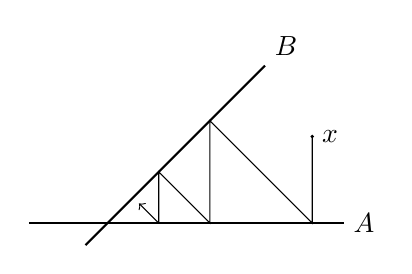
\begin{tikzpicture}
% A:
\draw[line width=.8pt] (-1,0) -- (3,0);
\draw (3,0) node[anchor=west]{$A$};

% B:
\draw[line width=.8pt] (-.28,-.28) -- (2,2);
\draw (2,2) node[anchor=south west]{$B$};

% x:
\draw[fill=black] (2.6,1.1) circle (.4pt);
\draw (2.6,1.1) node[anchor=west]{$x$};

% projections:
\draw (2.6,1.1) -- (2.6,0) -- (1.3,1.3) -- (1.3,0) -- (.65,.65) -- (.65,0);
\draw[->] (.65,0) -- (.4,.25);
\end{tikzpicture}
\end{center}
Let~$A$ and~$B$ be closed linear subspaces of~$H$
with projections~$Q$ and~$R$, respectively.
We consider the sequence
\begin{equation*}
Q,\ RQ,\ QRQ,\ RQRQ,\ \dotsc
\end{equation*}
Prove the following.
\begin{enumerate}
\item\label{5.24-1}
$QRQ\in\mathscr H$, $0\leq QRQ \leq I$.
%
\item\label{5.24-2}
For all $x\in H$ the sequence $QRQx$,  $QRQRQx$, 
$\dotsc$ converges.

Denote its limit by~$Px$.
We now have a map $P\colon H\ra H$.
%
\item\label{5.24-3}
$P$ is the projection onto $A\cap B$.
(If $QRQx=x$, then $x\in Q(H)$, so $Qx=x$.)
%
\item\label{5.24-4}
For every~$x$ the sequence
\begin{equation*}
Qx,\ RQx,\ QRQx,\ RQRQx,\ \dotsc
\end{equation*}
converges to~$Px$.
\end{enumerate}
\end{psec}
\end{document}
